
%%%%%%%%%%%%%%%%%%%%%%%%%%%%%%%%%%%%%%%%%%%%%%%%%%%%%
          %   \begin  CV und Beginn des Dokuments
%%%%%%%%%%%%%%%%%%%%%%%%%%%%%%%%%%%%%%%%%%%%%%%%%%%%
%\enlargethispage{3cm}

\chapter*{Albert Einstein}
\markboth{Albert Einstein}{Albert Einstein} % falls der CV über 2 Seiten geht um einen "Running Header" zu haben


\flushright
% Code mit Bild:
%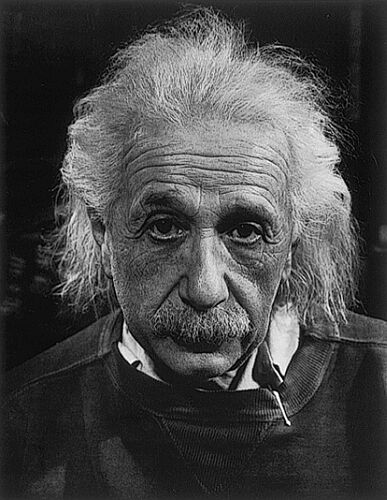
\includegraphics[scale=.2]{Abbildungen/albert-einstein.jpg}
%\vspace*{-5cm}{
%Code ohne Bild:
%\vspace*{-1cm}{
\subsection*{Persönliche Daten}
\flushleft
%\tabular-Umgebung
\normalsize
\begin{tabular}{lcl}
Adresse             & ~ & An der Kühruh 13\\
                    & ~ & 96123 Litzendorf\\[5pt]
Mobil               & ~ & 0170 - 9732890\\
Email               & ~ & sebastian.weller01@gmail.com\\[5pt]
Geburtsdatum        & ~ & 01.04.1992\\
Staatsangehörigkeit & ~ & deutsch\\
\end{tabular} 

\subsection*{Bachelorarbeit (optionaler Punkt)}
\begin{tabular}{lcl}
01/2016-07/2016     & ~~~~~ & Bachelorarbeit \\
                    & ~~~~~ & Ich bin das Thema der Bachelorarbeit\\[5pt]

\end{tabular} 
\\*  % Zeilenumbruch OHNE Seitenwechsel

\nopagebreak
\subsection*{Studium und Schulbildung}
\begin{tabular}{lcl}
01/2016 - 07/2016     & ~~~ &  Friedrich-Alexander-Universität Erlangen-Nürnberg\\
                      & ~~~ &  Hauptfächer Prokrastination und Bummelei\\
01/2010 - 01/2016     & ~~~ &  Albert-Einstein-Gymnasium, Erlangen\\
                      & ~~~ &  Leistungskurse: Feiern und Relaxen\\
\end{tabular}

\subsection*{Berufliche Erfahrungen / Praktika}
\begin{tabular}{lcl}
01/2016 - 07/2016     & ~~~ &  Wissenschaftlicher Hilfsmitarbeiter am Fraunhofer IIS\\
01/2016 - 07/2016     & ~~~ &  Praktikum bei Siemens Erlangen\\
\end{tabular}
\subsection*{Zusatzqualifikationen - (optional)}
\begin{tabular}{lcl}
Sprachen            &  & Deutsch (Muttersprache)\\
                    &  & Englisch (fließend in Wort und Schrift)\\
                    &  & Französisch (Grundkenntnisse)\\[5pt]
Programmiersprachen &  & Java \\
\end{tabular} 
\bigskip
\vspace*{.5cm}




Erlangen, den (Datum eintragen)\\*[20pt]\nopagebreak
\vspace{0.5cm}


\rule{5cm}{0.4pt}\\*\nopagebreak


Albert Einstein\\*\nopagebreak



